\appendix
\renewcommand{\thesection}{S\arabic{section}}

\section{Elasticity and pass-through grid}\label{supp:grid}

The regenerated grid spans $\varepsilon\in\{0.4,1,2,3\}$ and $\pi\in\{0.5,0.75,1\}$. Because only five displacement assignments are used per cell, it is an exploratory scaling diagnostic. Equal products $\varepsilon\pi$ generate equal deterministic wage-cut shocks; Bernoulli displacement outcomes vary across assignments. The grid is not an uncertainty interval.

\section{Reallocation sensitivity}\label{supp:reallocation}

The reallocation exercise uses five paired assignments and is exploratory.
Under the full schedule, the central 28.3 per cent penalty produces a mean
gross loss of \pounds\ReallocCentralGross\ million, Exchequer cost of
\pounds $\ReallocCentralExchequer\pm\ReallocCentralExchequerSD$ million,
cushioning of $\ReallocCentralCushion\pm\ReallocCentralCushionSD$ per cent,
and zero measured BHC-poverty change. With a three-month lag, gross loss
rises to \pounds\ReallocLagGross\ million and the Exchequer cost to
\pounds $\ReallocLagExchequer\pm\ReallocLagExchequerSD$ million. The 14 per
cent penalty gives gross loss of \pounds\ReallocLowPenaltyGross\ million and
Exchequer cost of
\pounds $\ReallocLowPenaltyExchequer\pm\ReallocLowPenaltyExchequerSD$
million. These pound levels are not commensurable with
the economy-wide wage-cut scenario because only selected movers' penalty is
removed.

\section{Observed-outturn stress scenario}\label{supp:measured}

The descriptive May 2025--February 2026 export window falls
\RealisedAggregateFall\ per cent against its two-year same-month baseline.
This is not a causal tariff estimate: it includes prices, exchange rates,
front-running, rerouting and other demand conditions.

The downside displacement scenario affects \MeasuredDisplacedWorkers\ thousand
weighted workers on average, is cushioned by
$\MeasuredDisplacedCushion\pm\MeasuredDisplacedCushionSD$ per cent and costs
the Exchequer
\pounds $\MeasuredDisplacedExchequer\pm\MeasuredDisplacedExchequerSD$ million.
The wage-cut scenario is cushioned by \MeasuredWageCushion\ per cent and costs
\pounds\MeasuredWageExchequer\ million. This is an observed-outturn downside
stress case, not a tariff-caused or preferred estimate; the validation
artifact also reports signed net exposure before expanding divisions are
clipped.

\section{HMRC destination-panel diagnostic}\label{supp:trade-panel}

Across \HMRCPanelProducts\ HS4 products, the capped value-weighted
specification estimates a \HMRCWeightedEffect\ per cent change in exports to
the US relative to the same products sent to the three comparison
destinations (95 per cent interval \HMRCWeightedCILower\ to
\HMRCWeightedCIUpper\ per cent, $p=\HMRCWeightedPValue$). Results have
similar signs against each destination, and May 2019--23 pseudo-policy
estimates are individually insignificant. This is not robust evidence of a
common product effect: equal product weights give \HMRCEqualEffect\ per cent
($p=\HMRCEqualPValue$), and restricting the sample to 2023 onward gives
\HMRCRecentEffect\ per cent ($p=\HMRCRecentPValue$). The estimated
differential trend is itself borderline ($p=\HMRCTrendPValue$). Most
importantly, broad steel and auto chapters fall \HMRCHighTariffEffect\ per
cent ($p=\HMRCHighTariffPValue$), compared with \HMRCOtherEffect\ per cent
for other products ($p=\HMRCOtherPValue$): the tariff-intensity ordering
fails. Figure~\ref{fig:hmrc-destination} displays the monthly gap. The panel
supports a post-policy decline concentrated in large US export products, but
it cannot attribute that decline to tariffs or validate the tariff-rate
mapping.

\begin{figure}[htbp]
\centering
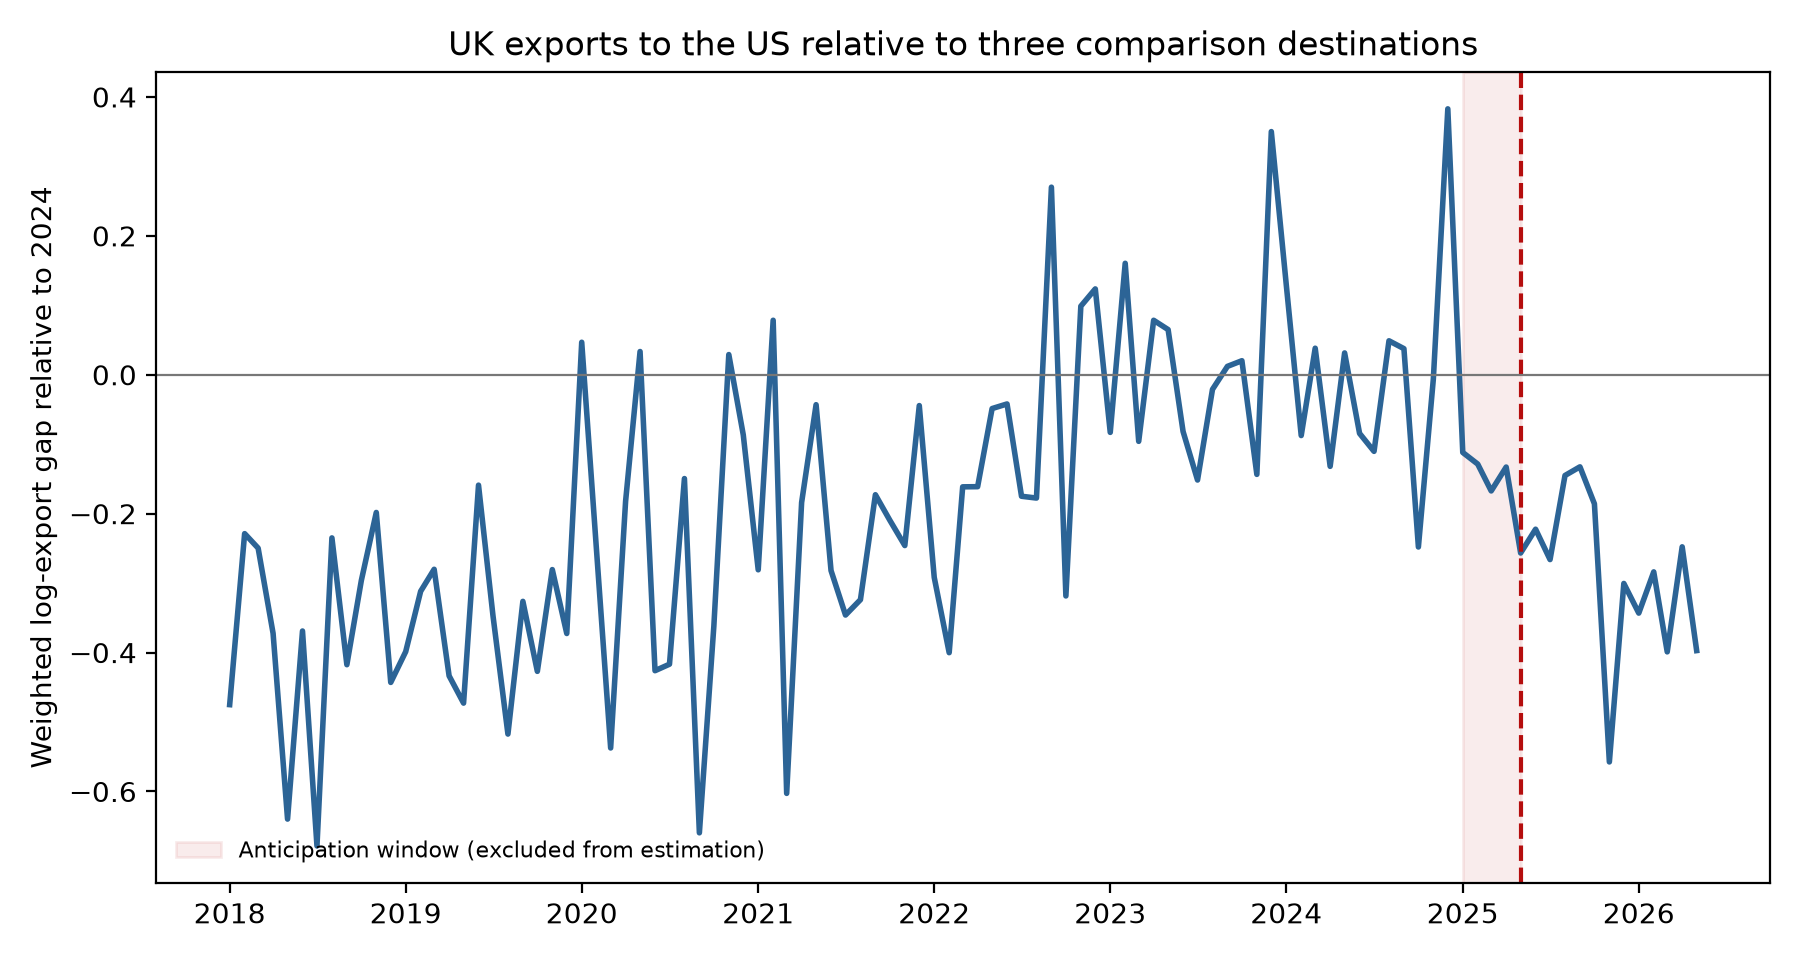
\includegraphics[width=.94\textwidth]{../results/figures/hmrc_destination_event_study.png}
\caption{Monthly capped-value-weighted gap between UK HS4 exports to the United States and mean exports of the same products to Canada, Japan and Australia, normalised to \HMRCFigureBase.}
\label{fig:hmrc-destination}
\end{figure}

The machine-readable specification, clustered standard errors, individual
destination checks, sample-start sensitivities, tariff-intensity groups and
May 2019--23 pseudo-policy estimates are stored in the event-study JSON
artifact; the plotted observations are stored in its companion monthly CSV.
Pre-policy
value weights are capped at the 99th percentile, giving an effective product
count of \HMRCPanelEffectiveProducts\ despite \HMRCPanelProducts\ included
HS4 products. Uncapped and equal-weight estimates disclose the remaining
concentration sensitivity.

\section{Economic Prosperity Deal counterfactual (withdrawn as a quantitative result)}\label{supp:epd}

On paired seeds, full minus EPD displacement differs by
$\EPDWorkerDifferenceThousands\pm\EPDWorkerDifferenceSDThousands$ thousand
workers, \pounds $\EPDGrossDifference\pm\EPDGrossDifferenceSD$ million of
gross earnings and \pounds $\EPDExchequerDifference\pm\EPDExchequerDifferenceSD$
million of annual Exchequer cost. The contrast is driven primarily by the
lower auto tariff and the exemption of pharmaceuticals in the EPD schedule,
and it should be interpreted as the fiscal value of changing the declared
sector shock while holding the household model and assignment draws fixed.
Two caveats withdraw it as a quantitative result. First, every paired
difference is comparable to or smaller than its own assignment
dispersion---the Exchequer contrast of \pounds\EPDExchequerDifference\
million carries an assignment SD of \pounds\EPDExchequerDifferenceSD\
million---so at the reported draw count the EPD contrast is not
distinguishable from allocation noise. Second, it prices a change in the
sector calibration whose own rank-order check fails; under the EPD schedule
the top-ten rank correlation is \RankCorrTopTenEPD. The comparison is
therefore retained as a qualitative illustration of the counterfactual
machinery, not as an estimate of the deal's value. It also does not include
quota allocation, above-quota trade, price responses, NHS pricing
concessions, or other general-equilibrium effects.
Figure~\ref{fig:epd-results} summarises the paired comparison. Autos drive
much of the difference; the scenario applies the in-quota rate to fixed
exposure without modelling quota allocation or future above-quota trade.

\begin{figure}[htbp]
\centering
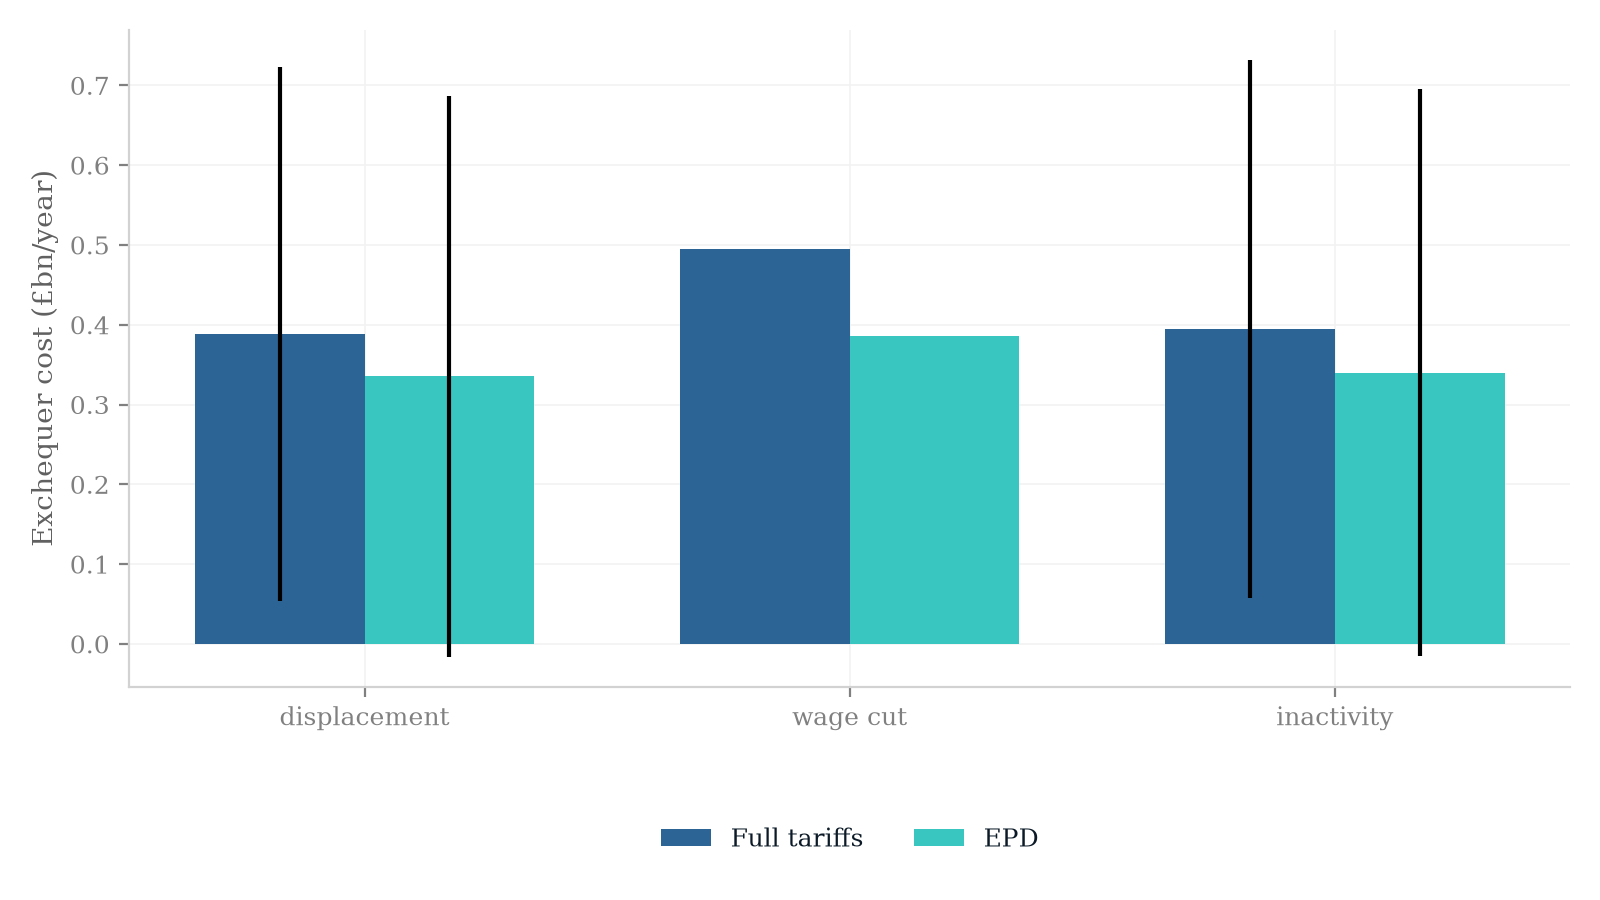
\includegraphics[width=.85\textwidth]{../results/figures/epd_counterfactual.png}
\caption{Full-schedule and EPD scenario comparison. Error bars are assignment standard deviations. The paired differences are comparable to or smaller than their assignment dispersion; no quantitative value should be placed on them.}
\label{fig:epd-results}
\end{figure}

\section{Demographic diagnostic}\label{supp:demographics}

The gender, age and household-type breakdown uses five Bernoulli assignments
and is exploratory. Selected exposed-sector workers are disproportionately men
and concentrated in prime and older working ages, but individual subgroup
estimates are too assignment-sensitive for precise rankings. The demographic
artifact is therefore a diagnostic rather than an inferential table.

\section{Supply-chain sensitivity}\label{supp:supplychain}

The input--output scenario adds upstream requirements using the ONS domestic Leontief inverse. The accounting shock has a 1.95 direct-plus-upstream factor. It is not a lower bound and is not multiplied by local-employment multipliers. In the exploratory ten-assignment microsimulation, displacement affects \SupplyChainDisplacedWorkers\ thousand weighted workers on average, costs the Exchequer \pounds $\SupplyChainDisplacedExchequer\pm\SupplyChainDisplacedExchequerSD$ million and raises relative BHC poverty by \SupplyChainDisplacedPoverty\ percentage points. The wage-cut variant costs \pounds\SupplyChainWageExchequer\ million and leaves measured relative poverty unchanged. Both runs predate the Universal Credit award-cache correction---a \FactorialCacheShift-point offset where it has been measured on the displacement margin---so their levels are not comparable with the main paper's bounds table; they are retained as an exploratory extension. These figures are accounting sensitivities, not all-channel causal estimates.

\section{Constituency machinery}\label{supp:constituency}

The enhanced-FRS constituency layer uses imputed industries rather than observed local industry structure. Its outputs are averaged over 20 paired worker-assignment draws (seeds 0--19), with each household's disposable-income change divided by household size before constituency means are constructed; the CSV artifact reports both the draw mean and the assignment-draw standard deviation. Because the constituency weights contain no observed local industry mix and the SIC imputation is held fixed, the outputs are synthetic demographic and income projections, not constituency exposure estimates. No map or seat-level figures are reported in the main paper; the machinery is documented here so that future work can populate it with observed local industry data.
